\documentclass[aspectratio=169,11pt]{beamer}
\usepackage{palermo-slides}
\addbibresource{references.bib}
\graphicspath{{figures/}}

\title{Entanglement percolation in\\random quantum networks}
\author{Alessandro Romancino}
\institute{Università degli Studi di Palermo}
\date{Seminar example \mydot Palermo}

\begin{document}

\maketitleslide
\maketoc[short]

\section{From quantum links to open bonds}

\begin{frame}{A link becomes an open bond}
  \begin{columns}
    \column{0.47\textwidth}
      % TikZ starting point. Replace the nodes and labels with your mechanism.
      \begin{tikzpicture}[control diagram]
        \node[box,fill=tlpink] (state) {$\lvert\psi_e\rangle$};
        \node[box,fill=tlblue,right=of state] (bond) {$B_e\in\{0,1\}$};
        \draw[arr] (state) -- node[lbl,above]{filter} (bond);
      \end{tikzpicture}

      \gap
      \capt{A successful local filter produces a maximally entangled pair.}
    \column{0.46\textwidth}
      \begin{math}
        \Pr(B_e=1\mid X_e)=X_e
      \end{math}

      \gap
      \capt{$X_e$ is the singlet-conversion probability of edge $e$.}

      \uncover<2->{%
        \biggap
        \schip{open bonds form usable paths}}
  \end{columns}

  \cite{2026romancinoa}
\end{frame}

\begin{frame}{The mean sets the classical threshold}
  \begin{columns}
    \column{0.51\textwidth}
      % PGFPlots starting point. Both illustrative distributions have mean 0.5.
      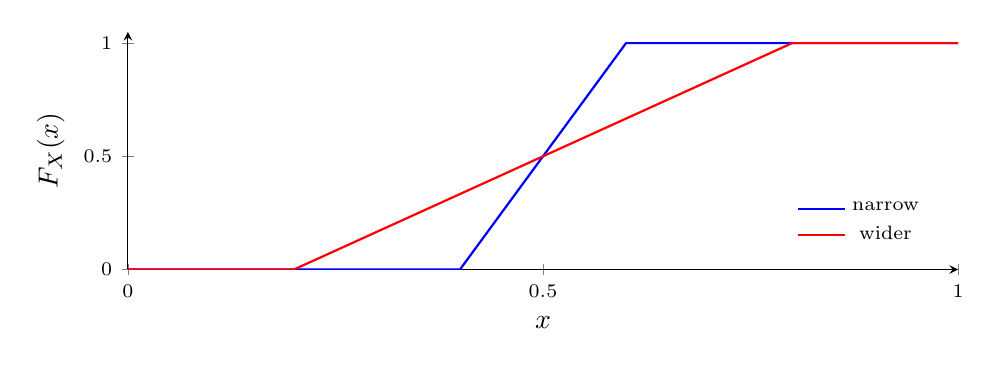
\begin{tikzpicture}
        \begin{axis}[
          width=\linewidth, height=4.6cm,
          axis lines=left,
          xmin=0, xmax=1, ymin=0, ymax=1.05,
          xtick={0,.5,1}, ytick={0,.5,1},
          xlabel={$x$}, ylabel={$F_X(x)$},
          tick label style={font=\scriptsize},
          legend style={font=\scriptsize,draw=none,at={(.97,.06)},anchor=south east}]
          \addplot+[thick,no marks] coordinates {
            (0,0) (0.2,0) (0.4,0) (0.6,1) (0.8,1) (1,1)
          };
          \addplot+[thick,no marks] coordinates {
            (0,0) (0.2,0) (0.4,0.333333) (0.6,0.666667) (0.8,1) (1,1)
          };
          \legend{narrow,wider}
        \end{axis}
      \end{tikzpicture}

      \capt{Illustrative distributions with the same mean}
    \column{0.43\textwidth}
      \begin{math}
        \Pr(B_e=1)=\mathbb E[X_e]
      \end{math}

      \gap
      \capt{Independent and identically distributed links give ordinary bond percolation.}

      \uncover<2->{%
        \biggap
        \schip[tyellow]{threshold at $\mathbb E[X_e]=p_{\mathrm c}$}}
  \end{columns}

  % Overlay 3 in the talk and a separate second page for this handout frame.
  \only<3|handout:2>{%
    \begin{tikzpicture}[remember picture,overlay]
      \fill[white,opacity=.78] (current page.south west)
        rectangle (current page.north east);
      \node[fill=tdark,text=white,rounded corners=6pt,inner sep=10pt,
            font=\large\bfseries] (takeaway) at (current page.center)
        {Equal means give the same classical threshold};
      \node[below=3mm of takeaway,fill=tlblue!45,inner sep=5pt]
        {The width of the distribution can matter for quantum protocols.};
    \end{tikzpicture}}

  \cite*{2026romancinoa}
\end{frame}

\section{Heterogeneous photonic links}

\begin{frame}{Polarization-dependent loss}
  \begin{columns}
    \column{0.51\textwidth}
      % Replace this box with your figure, using the line below.
      % \includegraphics[width=\linewidth,height=36mm,keepaspectratio]{device.pdf}
      \textcolor{tgray}{\fbox{%
        \parbox[c][34mm][c]{0.88\linewidth}{\centering
          Optical setup or device image\\
          \small\texttt{figures/device.pdf}}}}
    \column{0.43\textwidth}
      \begin{block}{A physical source of link disorder}
        Unequal attenuation changes the balance of the two polarization components.
      \end{block}

      \gap
      \capt{Different losses across links produce different singlet-conversion probabilities.}
  \end{columns}

  \cite{2026romancino}
\end{frame}

\begin{frame}{What sets the threshold?}
  \begin{columns}[T]
    \column{0.30\textwidth}
      \chip[tyellow]{Link model}

      \gap
      \capt{Each edge has a singlet-conversion probability drawn from a distribution.}

    \column{0.30\textwidth}
      \chip[tlblue]{Classical protocol}

      \gap
      \capt{For independent and identically distributed links, the mean determines bond occupancy.}

    \column{0.30\textwidth}
      \chip[tlpink]{Quantum preprocessing}

      \gap
      \capt{The $q$-swap strategy can lose its advantage as link disorder increases.}
  \end{columns}

  \cite*{2026romancinoa,2026romancino}
\end{frame}

\begin{frame}[standout]
  Questions and discussion
  % Optional acknowledgement or disclosure for your own talk.
  % \llm[Disclosure.]{Add the relevant details here.}
\end{frame}

\end{document}
